\documentclass[10pt]{beamer}

\usepackage{enumerate}
\usepackage{graphicx}
\usepackage{amsmath}
\usepackage{ragged2e}
\usepackage[latin1]{inputenc}
\usepackage[ngerman]{babel}
\usepackage{sidecap}

\mode<beamer>{
\usetheme[subsectionstyle=hide, compress]{Dresden}
\usecolortheme{sidebartab}
\setbeamertemplate{itemize subitem}[circle]
%\beamertemplatenavigationsymbolsempty
}


\title{Abschlusspr\"asentation PPG5}
\subtitle{WS 2009 / 2010}
\author{04. Februar 2010}
\date{Michele Collodo, Andreas Glossner, Karl-Christoph G\"odel, Bastian Hacker, Maria Obst, Alexander Wagner, David Winnekens}

\begin{document}

\frame
{
\titlepage
}

%%%%%%%%%%%%%%%%%%%%%%%%%%%%%%%%%%%%%%%%%%%%%%%%%%%%%%%%%%%%%%%%%%%%%%%%%%%%%%%%%%%%%%%%%%%%%%%%%%%%%%%%%%%%%%%%
\section{LED-Spektrometer}
\subsection[]{Grundidee}
\frame
{
\frametitle{Grundidee}
\begin{figure}
\begin{center}
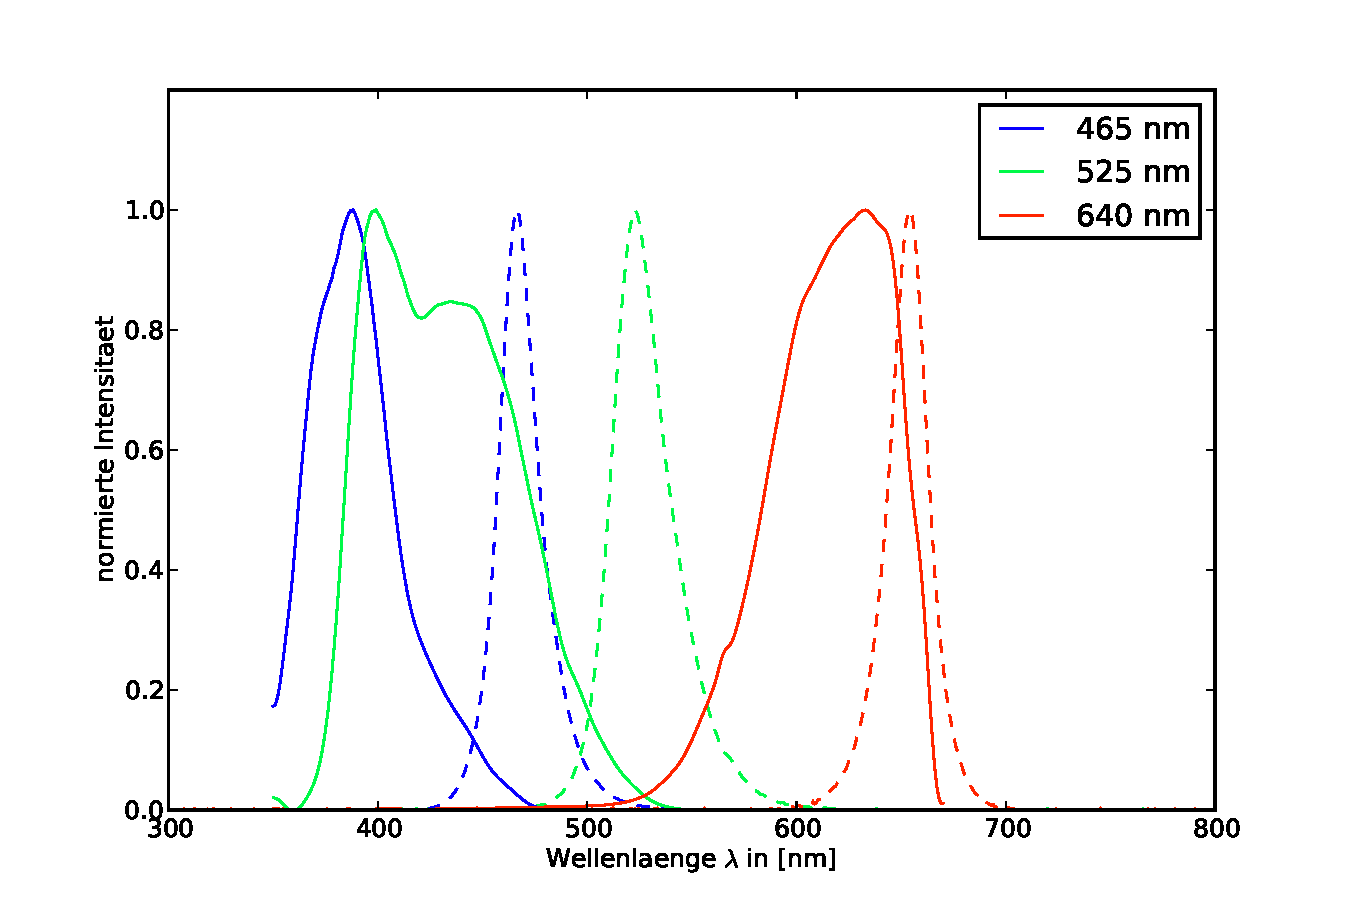
\includegraphics[width=0.8\textwidth]{./images/absorp-emit.pdf}
\caption{Verschiedenfarbige LEDs mit verschiedenen Absorptionsspektren}
\end{center}
\end{figure}
}

\subsection[]{Vorgehen}
\frame
{
\frametitle{Vorgehen}
\begin{enumerate}
\item Vormessungen
\item Elektronik
\item Software 
\end{enumerate}

\begin{figure}
\begin{center}
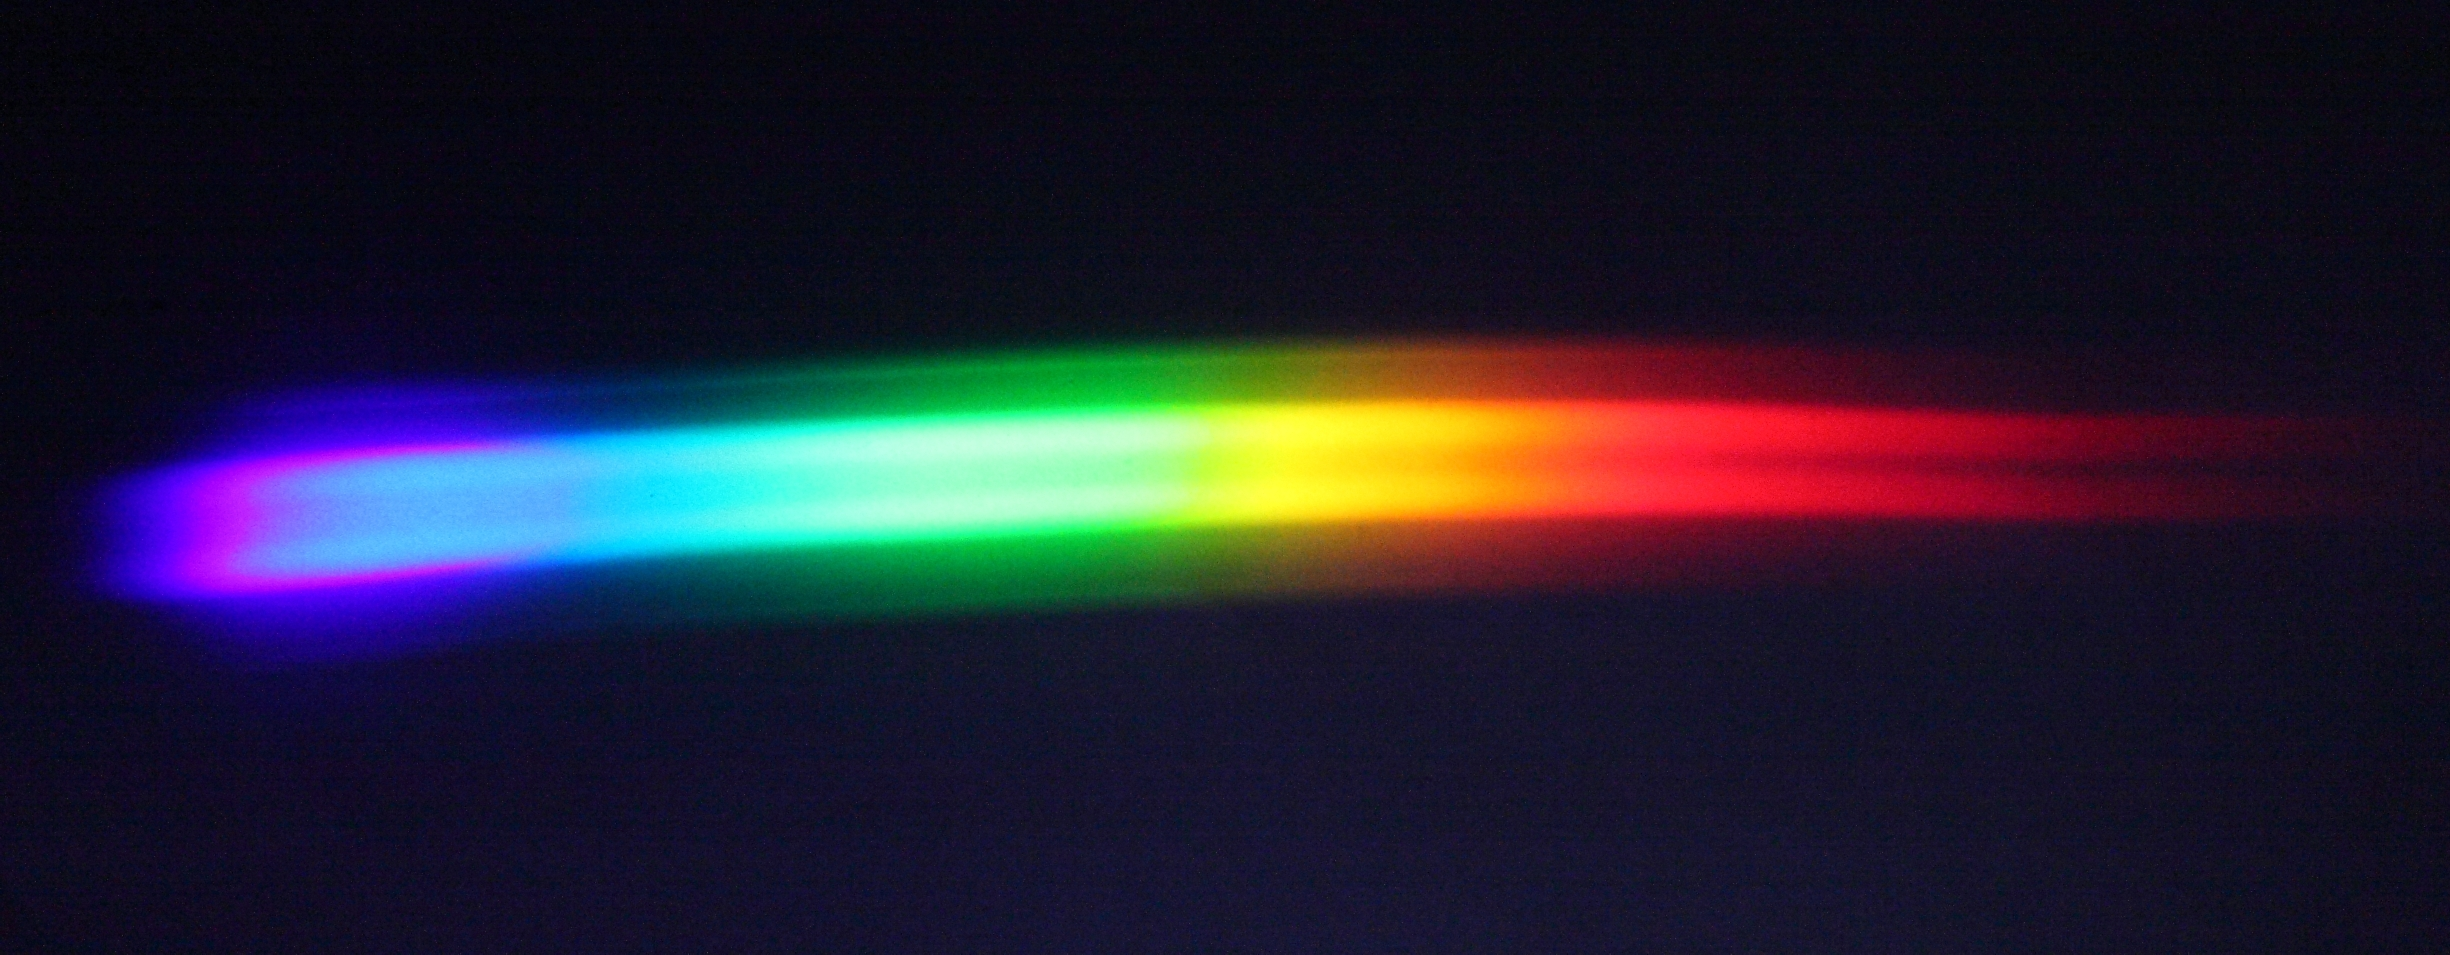
\includegraphics[width=\textwidth]{./images/spektrum_web.jpg}
\end{center}
\end{figure}
}
\frame
{
\frametitle{Vormessungen I}
\begin{figure}
\begin{center}
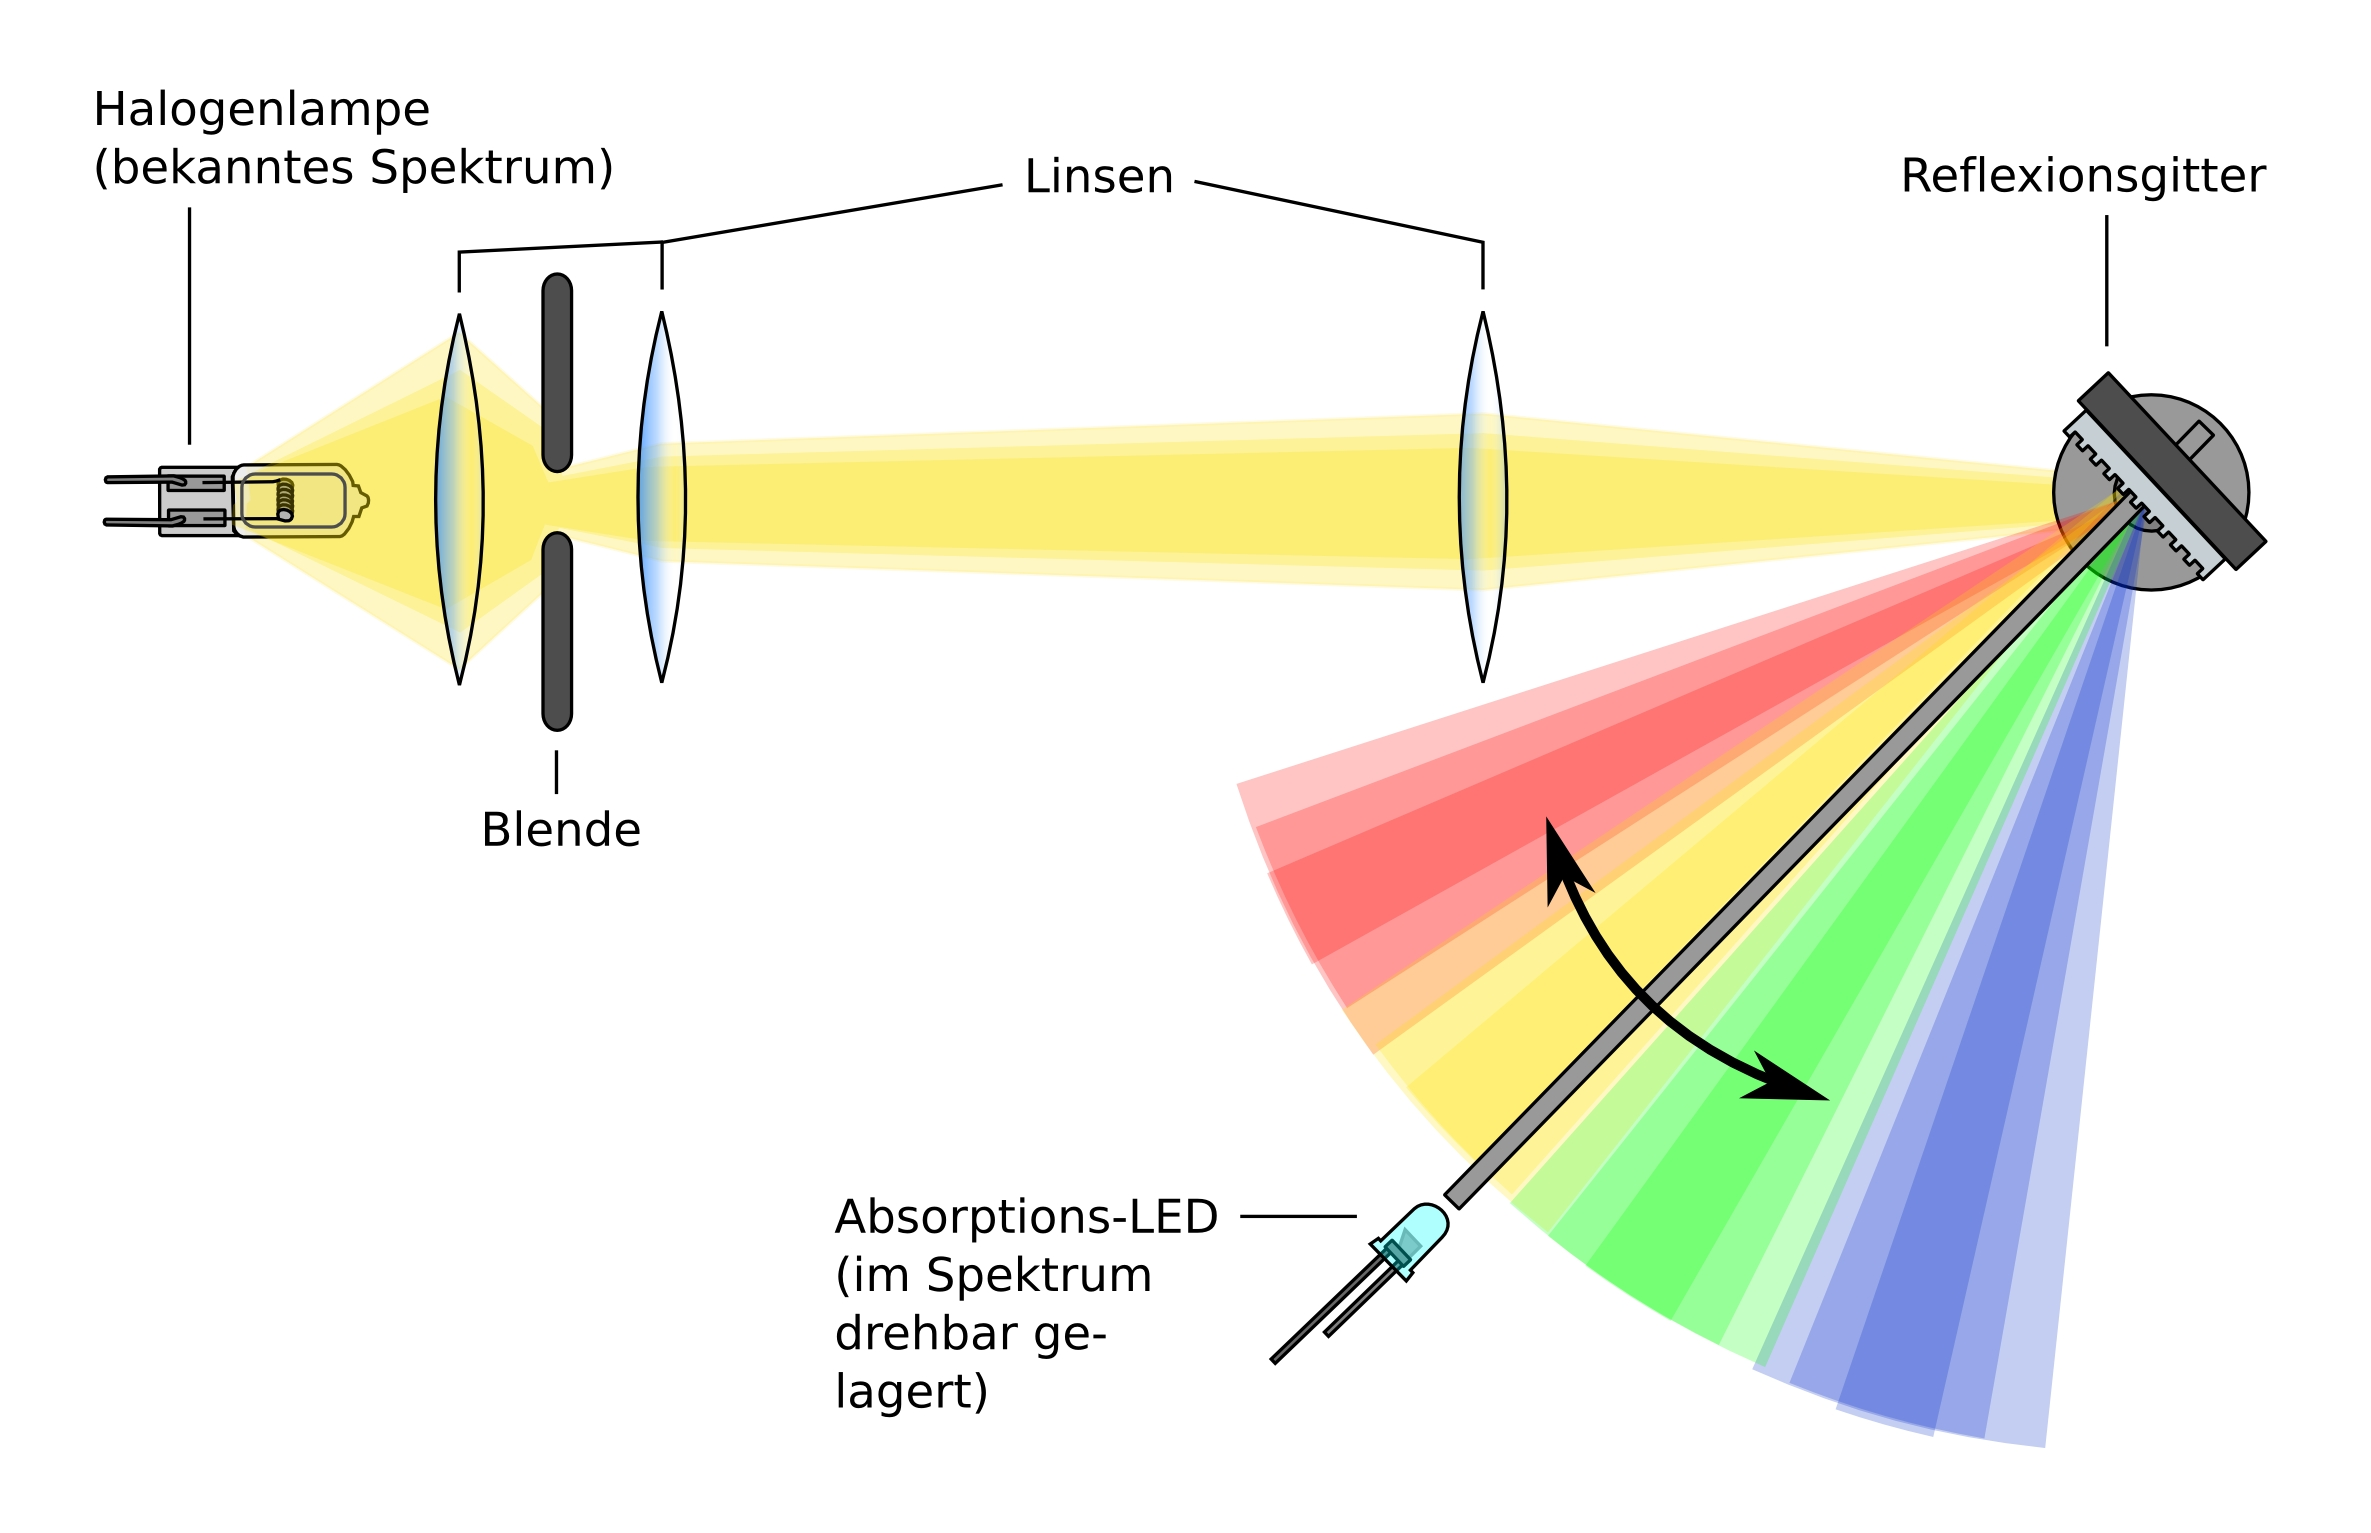
\includegraphics[width=0.8\textwidth]{./images/setup.jpg}
\caption{Aufbau f\"ur die Kalibration}
\end{center}
\end{figure}
}
\frame
{
\frametitle{Vormessungen II}
\begin{figure}
\begin{center}
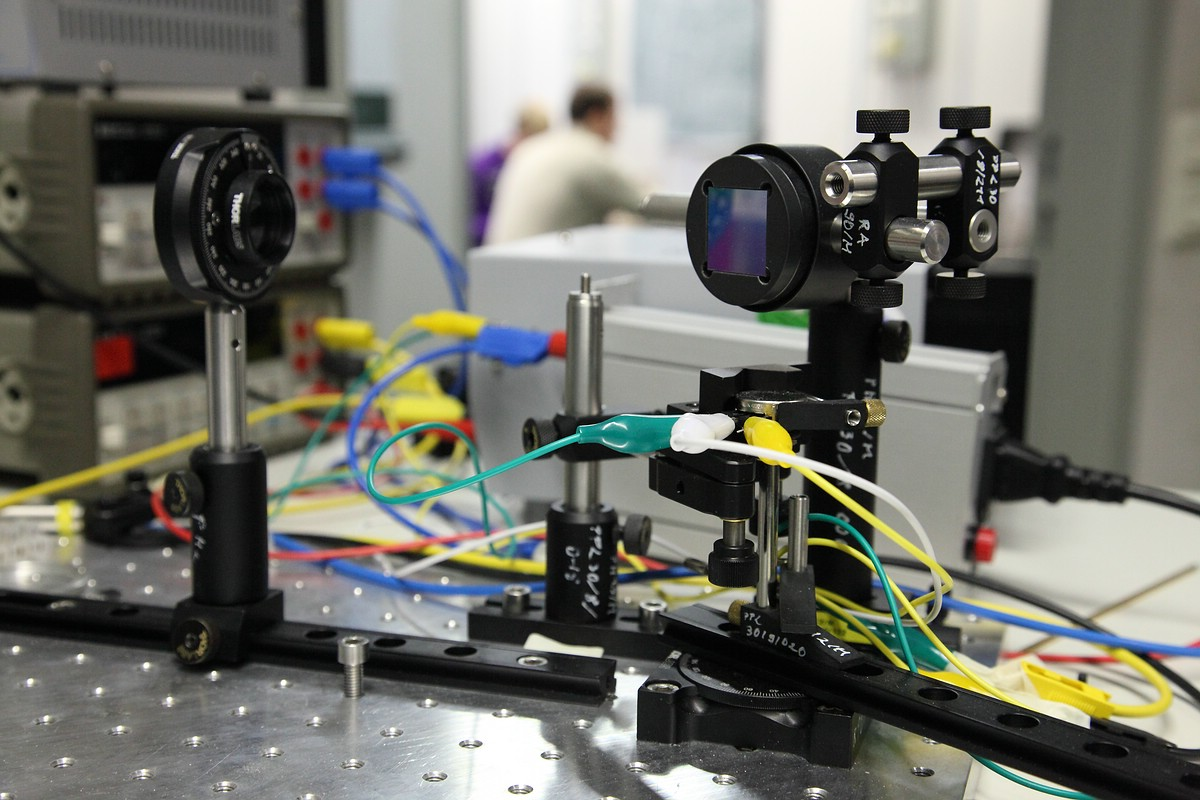
\includegraphics[width=0.8\textwidth]{./images/prIMG_7244}
\caption{kontinuierliche Winkelmessung}
\end{center}
\end{figure}
}
\frame
{
\frametitle{Elektronik I}
\begin{figure}
\begin{center}
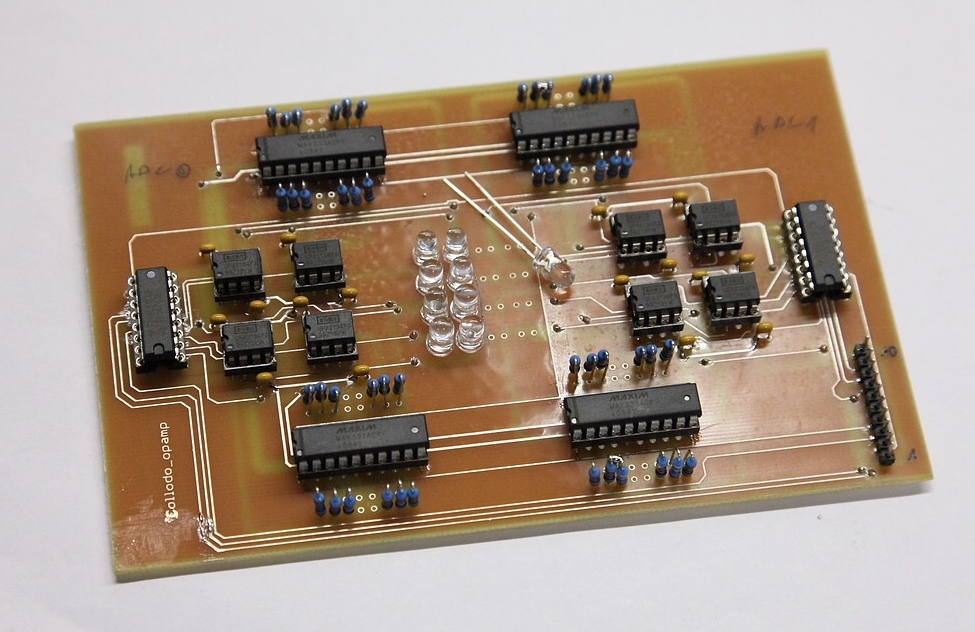
\includegraphics[width=0.8\textwidth]{./images/prIMG_7253crop.jpg}
\caption{Fertige Platine}
\end{center}
\end{figure}
}
\frame
{
\frametitle{Elektronik II}
% Schaltplan einfuegen
schaltplan
}
\frame
{
\frametitle{Software}
flussdiagramm
}
\subsection[]{Ergebnisse}
\frame
{
\frametitle{Ergebnisse}
laberlaber
}

%%%%%%%%%%%%%%%%%%%%%%%%%%%%%%%%%%%%%%%%%%%%%%%%%%%%%%%%%%%%%%%%%%%%%%%%%%%%%%%%%%%%%%%%%%%%%%%%%%%%%%%%%%%%%%%%
\section{Andere Projekte}
\subsection[]{Gr\"atzelzelle}
\frame
{
\frametitle{Gr\"atzelzelle}
\begin{figure}
\begin{center}
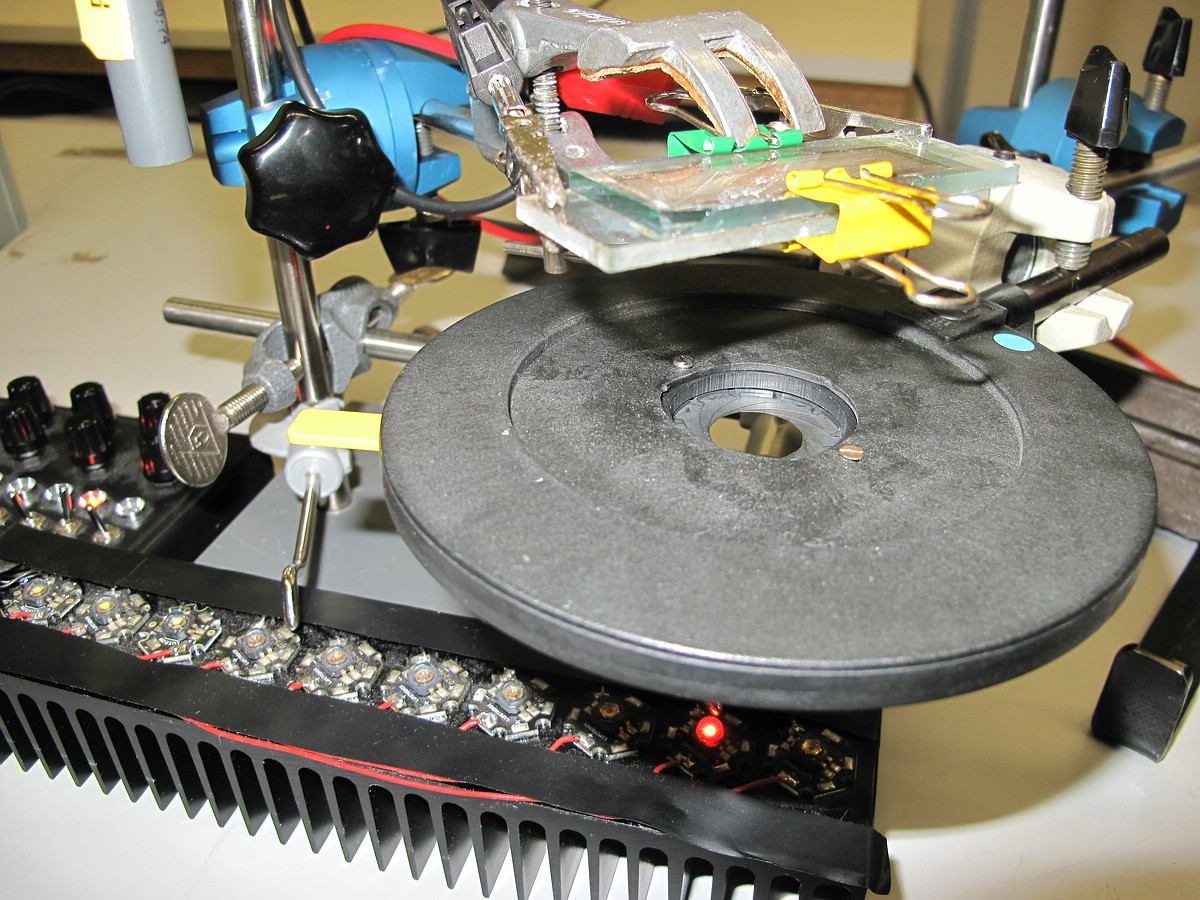
\includegraphics[width=0.7\textwidth]{./images/prIMG_3497.jpg}
\caption{Gr\"atzelzelle, beleuchtet von einer LED}
\end{center}
\end{figure}
}
\subsection[]{MHD-Generator}
\frame
{
\frametitle{MHD-Generator}
\begin{figure}
\begin{center}
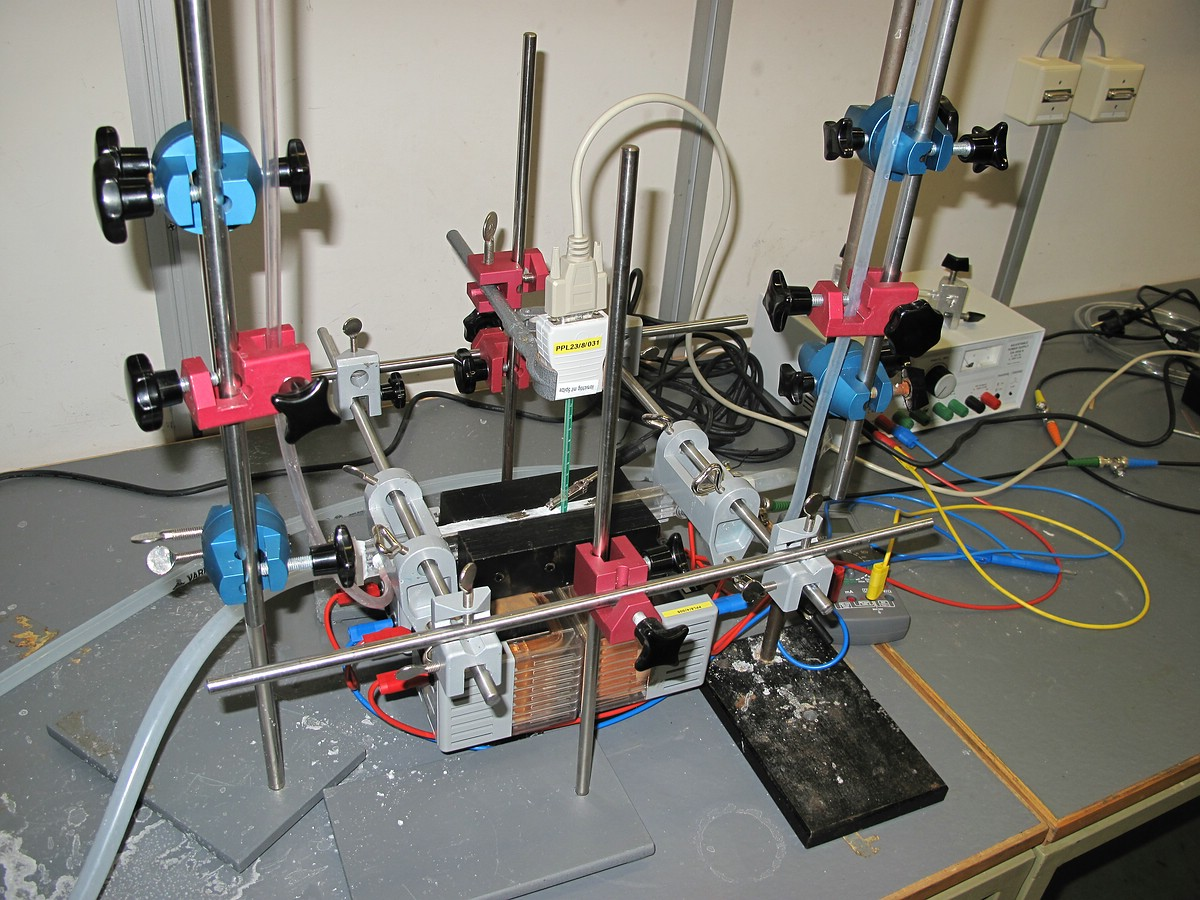
\includegraphics[width=0.7\textwidth]{./images/prIMG_3768.jpg}
\caption{MHD-Generator mit Zelle im Magnetfeld}
\end{center}
\end{figure}
}
\subsection[]{Erdrotation}
\frame
{
\frametitle{Erdrotation}
%\begin{SCfigure}
\begin{figure}
\begin{center}
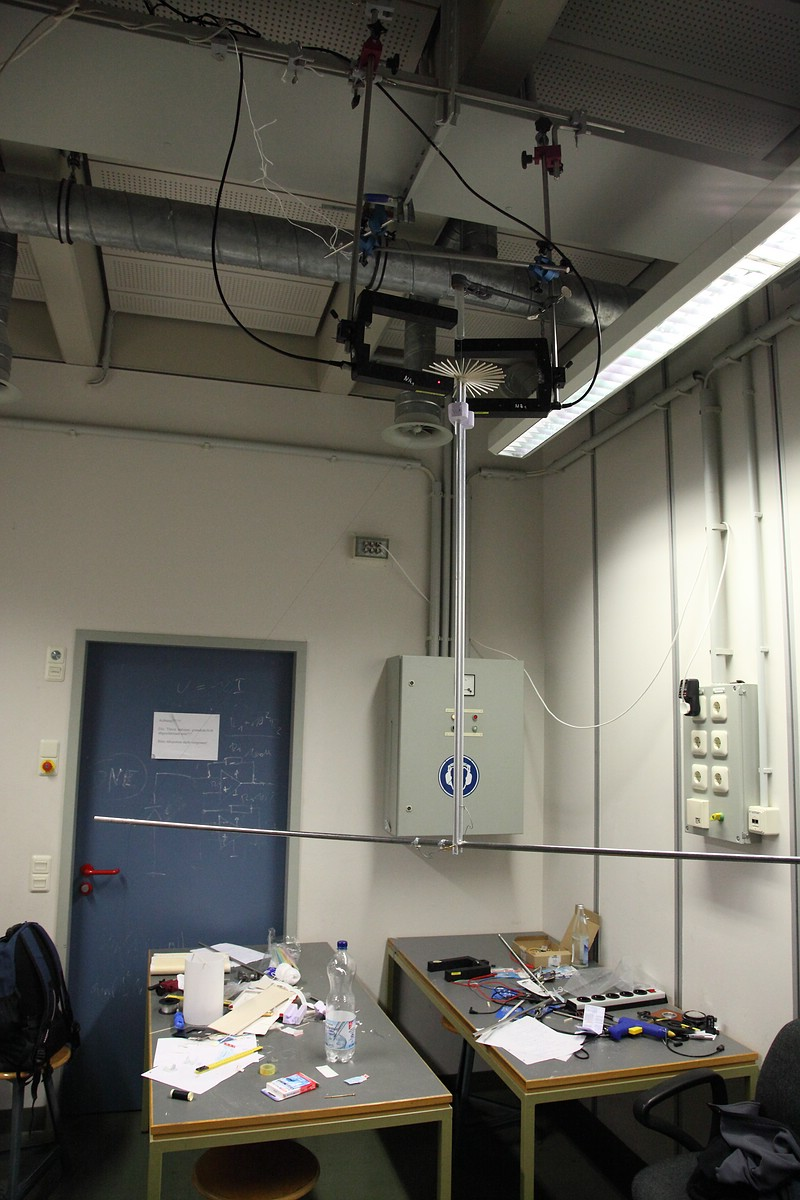
\includegraphics[width=0.4\textwidth]{./images/prIMG_7266.jpg}
%\caption{Pendel zur Messung der Erdrotation}
%% des geht noch net wirklich, entweder des endgueltige bild is quer oder ich ueberleg mir dann was wenns so weit is...
\end{center}
\end{figure}
%\end{SCfigure}
}

\end{document}
